%! TeX program = lualatex
%---------------------------ALLGEMEINE IMPORTS-------------------------------------
\documentclass[12pt,english,ngerman]{scrartcl}
\input{./protokoll_template/template.latex/input/shared_preamble.tex}

% Kopfzeile
\ihead{WS22\\
	29.03.2023} \chead{\textsc{Stark} Matthias - 12004907 \\
	\textsc{Philipp} Maximilian - 11839611}
\ohead{Röntgenfluoreszenzanalyse \\ 
%FLAB 2 \\
Compton-Effekt}

% Fußzeile
%todo
%\addbibresource{SolarWirkungsgrad.bib}

\usepackage{luacode}

\DeclareSIUnit\px{px}
\DeclareSIUnit\strich{|||}
\DeclareSIUnit\Var{var}
\DeclareSIUnit\VA{VA}
\DeclareSIUnit\bar{bar}

\usepackage{cleveref}

\crefname{enumerate}{Aufzählung}{Aufzählungen}

\begin{document}

\begin{luacode*}
	dofile("createExtraPDF.lua")
\end{luacode*}

%todo
%
\includepdf{./deckblatt.pdf}
\tableofcontents

\newpage

\section{Aufgabenstellung\label{Auf}}

\subsection{Röntgenfluoreszenzanalyse}

Im Zuge des Beispiels Röntgenfluoreszenzanalyse sind folgende Versuche durchzuführen:

\begin{itemize}
	\item Aufnahme und Kalibrierung eines Röntgenenergiespektrums
	\item Zeigen der Gültigkeit des Moseleyschen Gesetzes anhand der bereitgestellten Metalle und 
	Ermittlung der Abschirmkonstante der K-Linien
	\item Analyse der Zusammensetzung von unbekannten Proben
\end{itemize}

\subsection{Compton-Effekt}

Ziel dieses Versuchs ist die Messung der Energie der gestreuten Photonen in Abhängigkeit vom Streuwinkel. 
Dabei werden folgende Punkte durchgeführt:

\begin{itemize}
	\item Aufnahme des Primärspektrums und Energiekalibrierung des Detektors
	\item Aufnahme der Spektren in Streuanordnung
	\item Bestimmung der Energie als Funktion des Streuwinkels
\end{itemize}


\section{Grundlagen}\label{Grund}


\subsection{Röntgenfluoreszenzanalyse}


\subsection{Compton-Effekt}



\section{Versuchsanordnung}\label{sec:versuchsanordnung}

Für beide Teile des Versuchs wird das Röntgengerät aus \autoref{fig:aufabau} verwendet.
Zunächst wird die Stromversorgung
und die Verbindung zum PC mittels Cassy Lab hergestellt. Nun wird mit den Drehschaltern eine
Spannung von \SI{30.0(2)}{\kilo eV} und ein Strom von \SI{1.00(2)}{mA} eingestellt.
Nach richtigen SChließen der Tür wird die Röntgenstrahlung mit dem HV Knopf kurz eingeschaltet,
um zu überprüfen, ob das Gerät funktioniert.

\begin{figure}[H]
	\begin{center}
		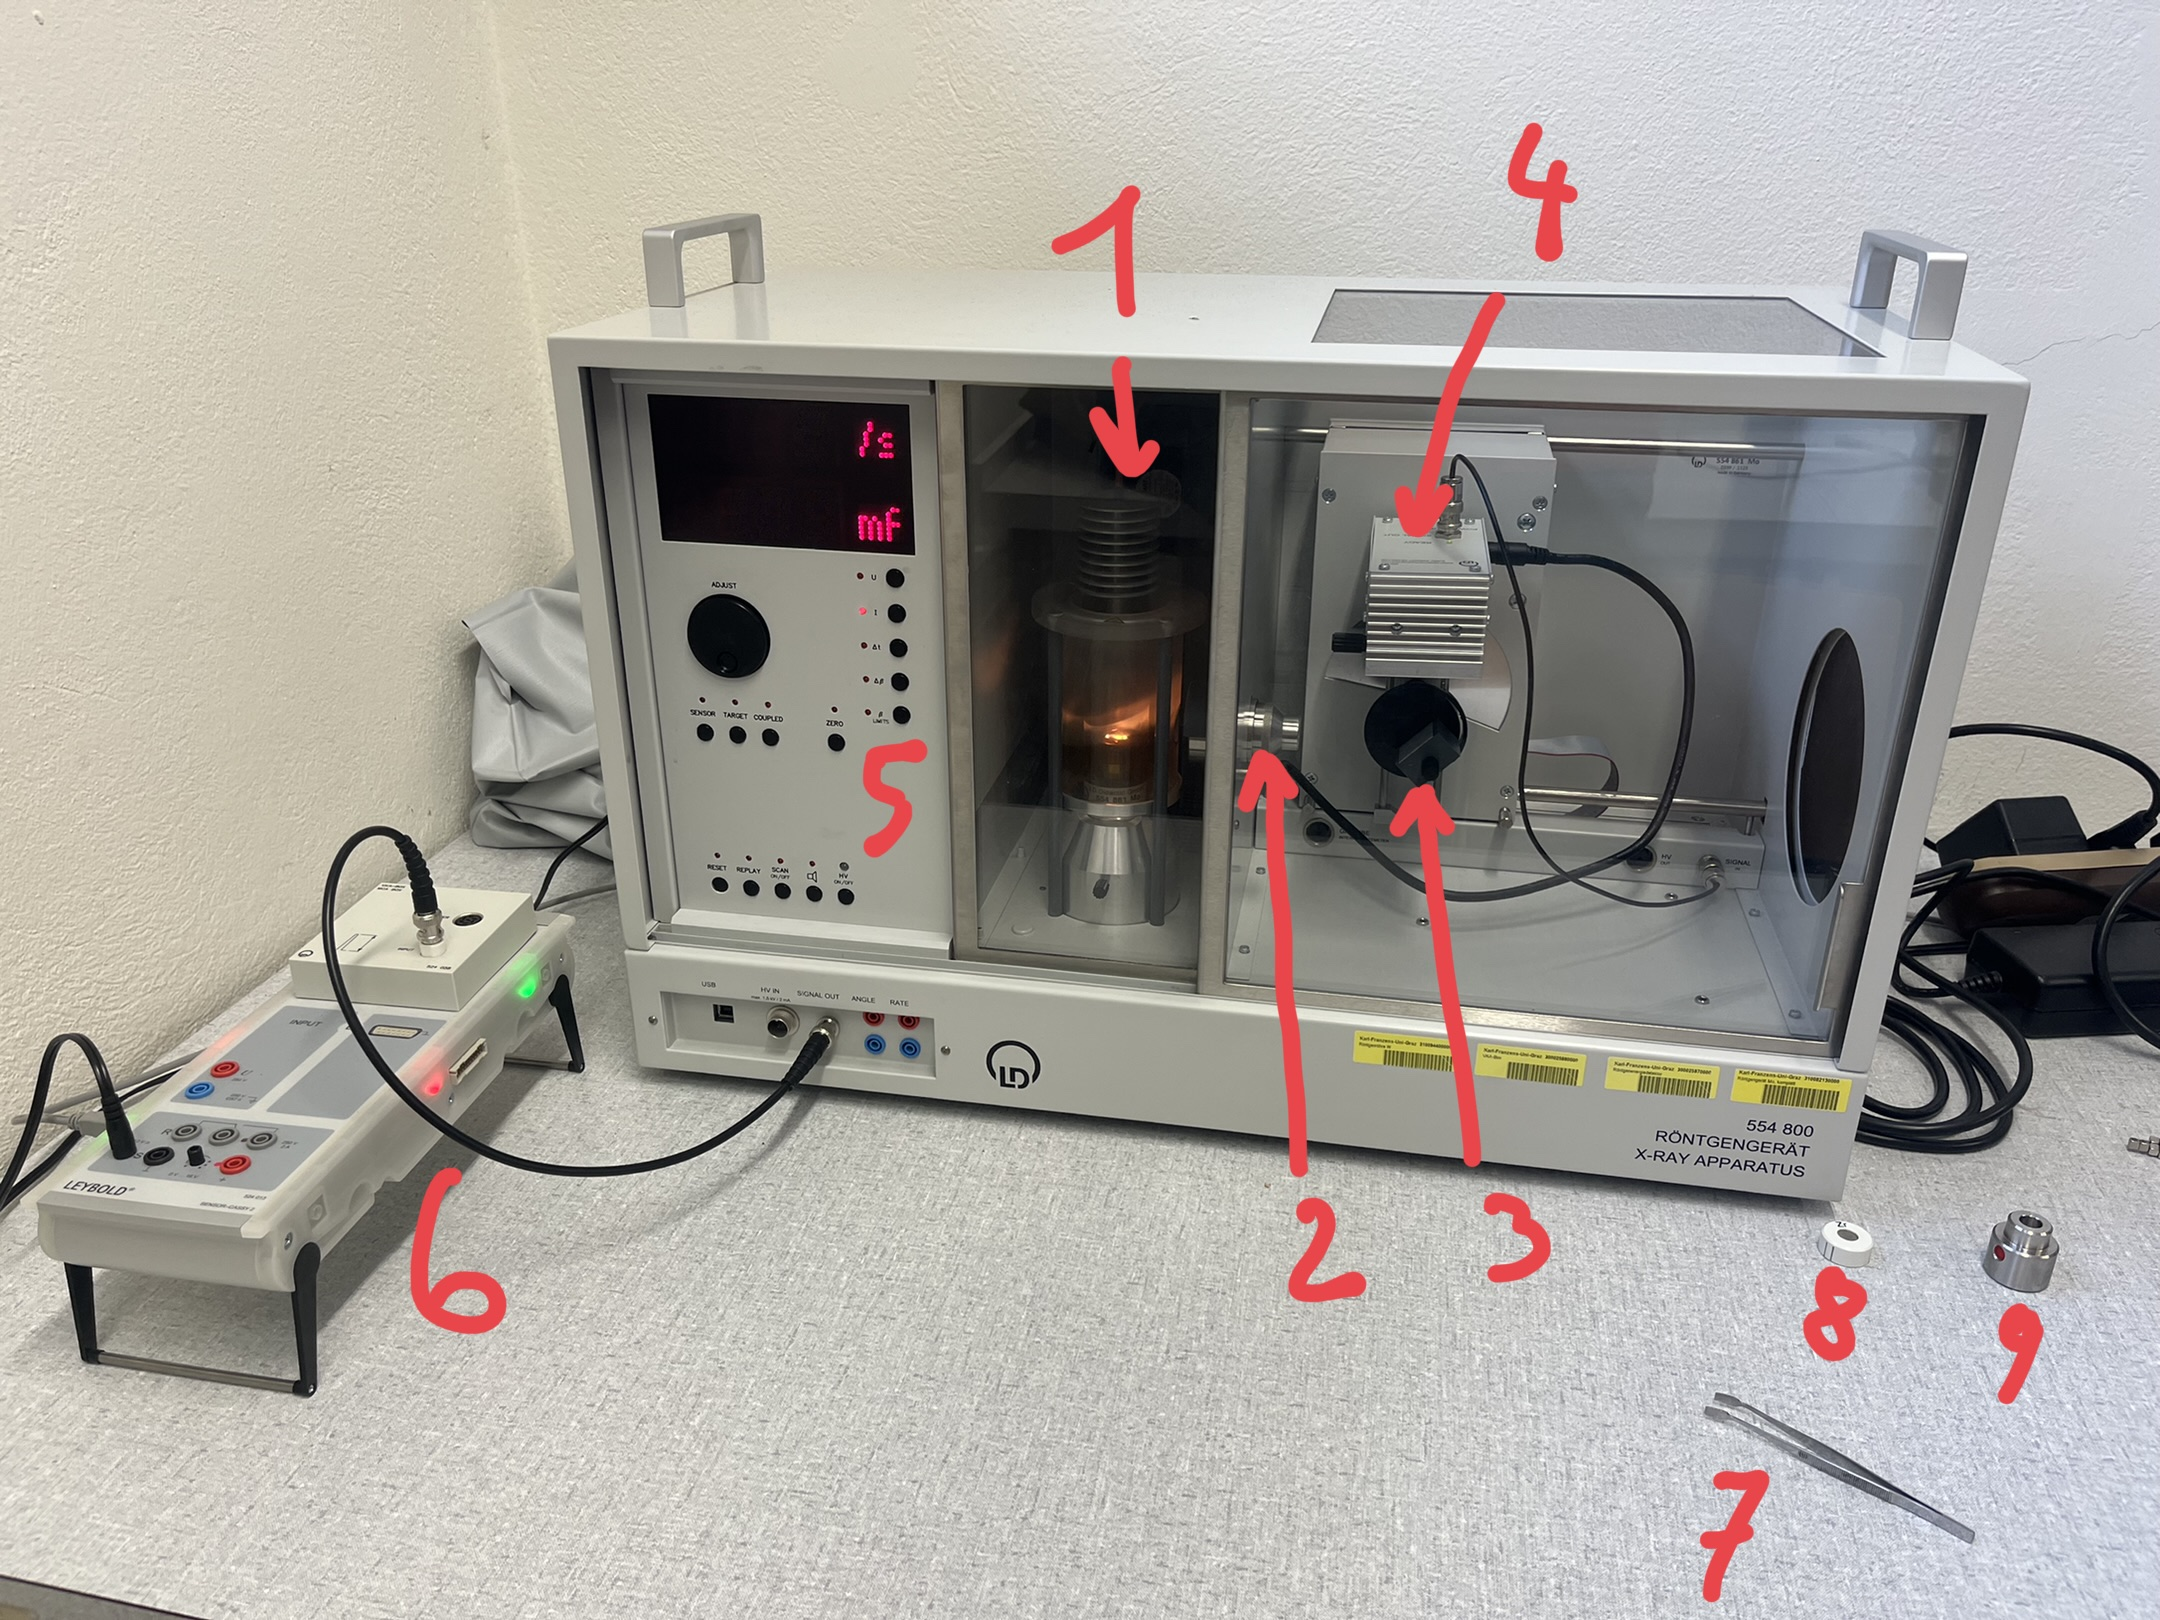
\includegraphics[width =0.8\textwidth]{./figures/aufbau.jpg}
	\end{center}
	\caption[Verwendetes Röntgengerät]
	{Verwendetes Röntgengerät\\
	1 \dots Röherenraum mit Röntgenröhre\\
	2 \dots Kollimator\\
	3 \dots Targetarm mit Targettisch auf Goniometer\\
	4 \dots Sensor auf Goniometer\\
	5 \dots Bedienfeld mit Drehschalter für alle Einstellungen\\
	6 \dots Cassy Lab 2\\
	7 \dots Pinzette für Probenwechsel\\
	8 \dots Zr- Filter\\
	9 \dots Abschwächerblende
	}\label{fig:aufabau}
\end{figure}

\subsection{Röntgenfluoreszenzanalyse}

Zunächst werden die Abstände zwischen Kollimator und Target bzw. zwischen Target und Sensor eingestellt, damit diese 
5 - 6 cm betragen. Dies geschieht manuell durch Lockerung der entsprechenden Schraube und Bewegung des Bauteils auf den
Führungsschienen.
Nun werden die Winkel des Targetarms und 
des Senosors eingestellt. Wichtig ist dabei, dass dies elektrisch, über die entsprechenden Knöpfe geschieht.
Der Winkel des Targets wird dabei auf \SI{45.0(2)}{\degree} eingestellt, der des Sensors auf \SI{90.0(2)}{\degree}.
Mit der "Zero"-Taste können die Winkel zurück in die Ausgangsposition gebracht werden.

\subsection{Compton-Effekt}

Für diesen Teil des Versuchs wird der Zr-Filter (siehe 8 in \autoref{fig:aufabau}) verwendet.
Dieser wird über den Metalbolzen des Kolimators geschoben, bevor dieser in seine Einbuchtung gesteckt wird.
Für die Aufnahme des Kalibrierungsspektrums wird zusätzlich noch die Abschwächerblende verwendet. Diese wird 
über den Kolimator geschoben, wie in \autoref{fig:abschwacheblende} sichtbar. Zusätzlich wird für
die Kalibration auch der Targethalter ausgebaut.


\begin{figure}[H]
	\centering
	\captionbox[Montierte Abschwächerblende]{Montierte Abschwächerblende\label{fig:abschwacheblende}}{
		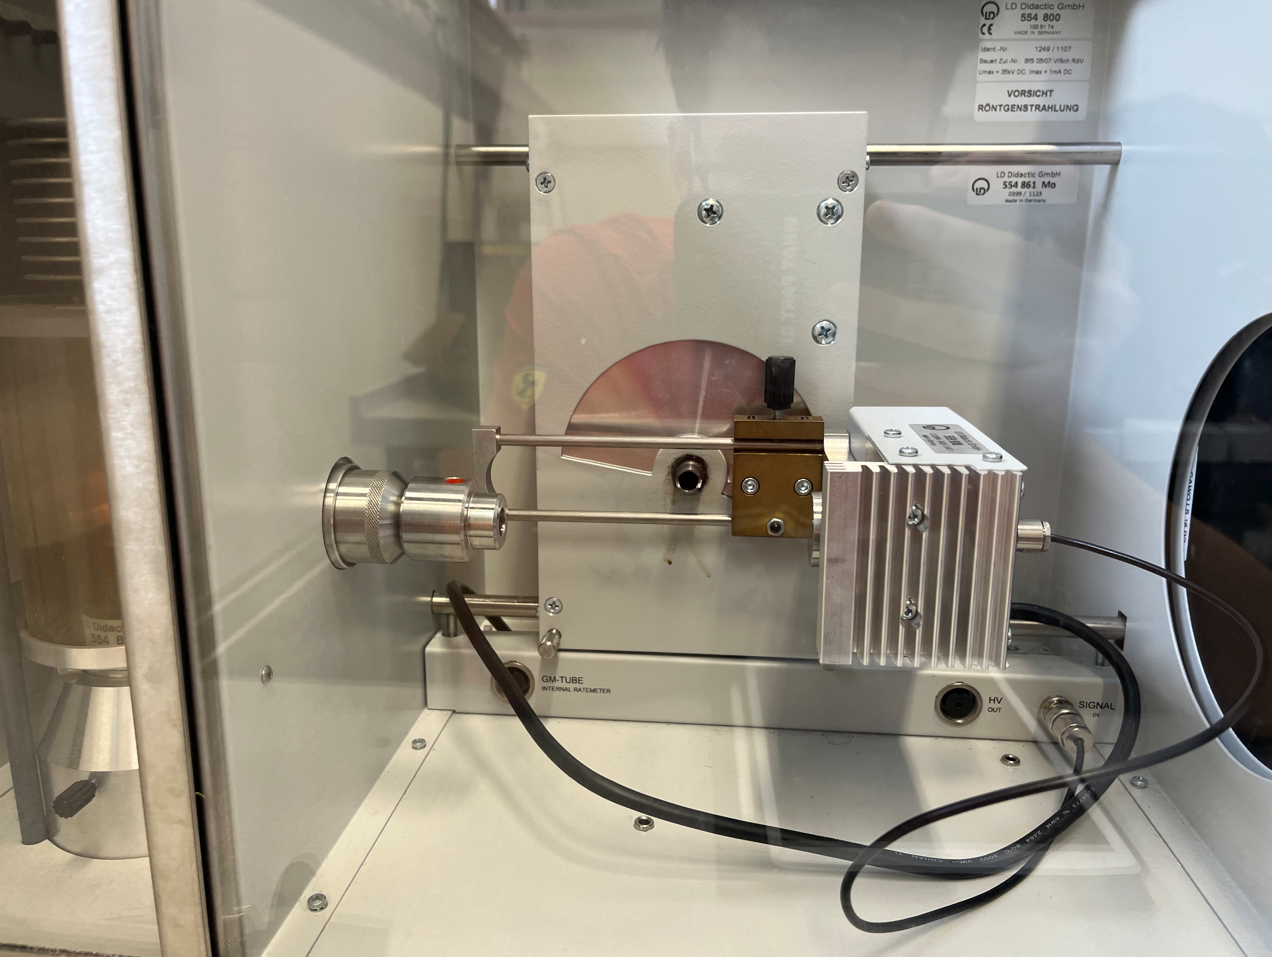
\includegraphics[width=.45\textwidth]{./figures/blende.PNG} } \hfill
	\captionbox[Maximale Auslenkung des Sensors]{Maximale Auslenkung des Sensors\label{fig:auslenkung}}{
		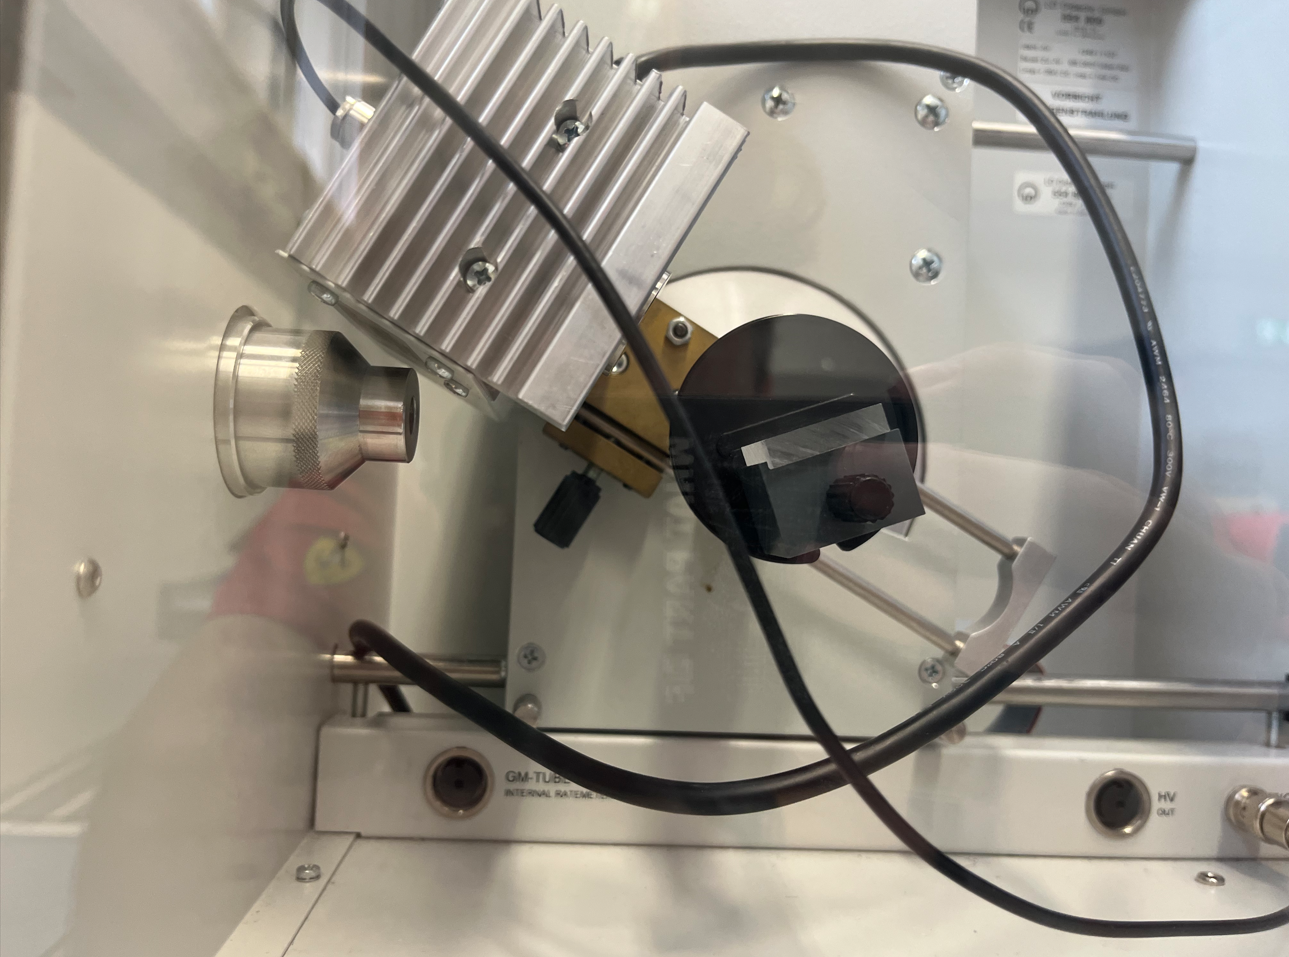
\includegraphics[width=0.45\textwidth]{./figures/auslenkung.PNG} }
\end{figure}


Für die Messung der Streuwinkel wir die Abschwächerblende wider entfernt und der Targethalter eingebaut. 
Bezüglich der Abstände von Sensor und Targethalter wird darauf geachtet, dass ein Schwenken von bis zu 
\SI{150.0(2)}{\degree} möglich ist, wie in \autoref{fig:auslenkung} sichtbar.


\section{Geräteliste}\label{sec:geraeteliste}

%todo

Für die Elektronen-Spin-Resonanz werden die in \autoref{tab:gerate_spin} aufgelisteten
Geräte verwendet.

\begin{table}[H]
	\caption{Verwendete Geräte für die Elektronen-Spin-Resonanz
	}
	\begin{tblr}{cells={font=\footnotesize},colspec={lllll}}
			\textbf{Gerätetyp}    & \textbf{Hersteller} & \textbf{Typ}     & \textbf{Inventar-Nr} & \textbf{Anmerkung}              \\
			ESR-Grundgerät        & KFU Graz            & Rep-Art-Onl-1066 & REP103801            &                                 \\
			ESR-Betriebsgerät     & Leybold             & 514571           &                      & mit Amperemeter                 \\
			Zweikanal Oszilloskop & Hameg               & HM205-2          & DOZ-3                & analog                          \\
			Helmholzspule         & LD                  & 555604           &                      & 2 x                             \\
			Steckspulen           &                     &                  &                      & mit unterschiedlichen Windungen \\
			Graphitprobe          &                     &                  &                      &                                 \\
			Sockel                &                     &                  &                      &                    \\
			Kabel                 &                     &                  &                      & BNC und Banane                 
	\end{tblr}\label{tab:gerate_spin}
\end{table}



\section{Versuchsdurchführung und Messergebnisse}\label{sec:versuchsdurchfuehrung_messergebnisse}

\subsection{Röntgenfluoreszenzanalyse}

\subsubsection{Aufnahme des Kalibrierungsspektrums}

Nachdem der Versuchsaufbau, wie bereits in \autoref{sec:versuchsanordnung} erklärt, durchgeführt wurde,
wird zunächst das Kalibrierungstarget aus die entsprechende Position gelegt. Dabei handelt es sich um 
ein verzinktes Eisenblech. Nun werden die Winkel des Targets und des Sensors richtig eingestellt und der
Sensor über das Cassy Lab 2 mit dem Computer verbunden.
In der Computersoftware werden unter den Messparametern die Einstellungen 
"Vielkanalmessung, 512 Kanäle, negative Pulse, Verstärkung = -2,5, Messdauer = 300 s“
eingegeben. Nun kann der Röntgenstrom eingeschaltet und die Messung gestartet werden.

Nun müssen den zwei erzeugten Peaks die entsprechenden Energien zugeordnet werden. 
Für Fe ist die entsprechende Energie \SI{6.40}{keV} und für Zn \SI{8.64}{keV} \cite{unterlagen_rontgenfluorenzenz}.
Das erzeugte Kalibrierungsspektrum ist in \autoref{fig:kalibrierung_rontgenfluoreszenz} sichtbar.

%todo fig:kalibrierung_rontgenfluoreszenz

\subsubsection{bereitgestellte Metalle}

Nachdem das Kalibrierungsspektrum aufgenommen wurde werden nun die verschiedenen Proben auf den Targethalter gelegt 
und die Messung, wie bereits zuvor für die Kalibreirung beschrieben, durchgeführt. Beim Wechseln der Proben ist zu beachten, 
dass die Röntgenstrahlung immer ausgeschalten ist, wenn die Tür geöffnet wird. Auch muss die Röntgenstrahlung kurz 
eingeschaltet werden bis die Glühkathode einen konstanten Farbverlauf aufweißt, bevor die Messung gestartet wird.
Die so erzeugten Diagramme der einzenen Proben sind in folgenden Abbildungen immer mit dem Referenzspektrum sichtbar.

%todo alle diagramme

\subsubsection{unbekannte Probe}

Nun werden zwei eigene Proben, sichtbar in \autoref{fig:unbekannte_pr}, auf den Targethalter gelegt, um deren genaue Zusammensetzung zu bestimmen.

\begin{figure}[H]
	\begin{center}
		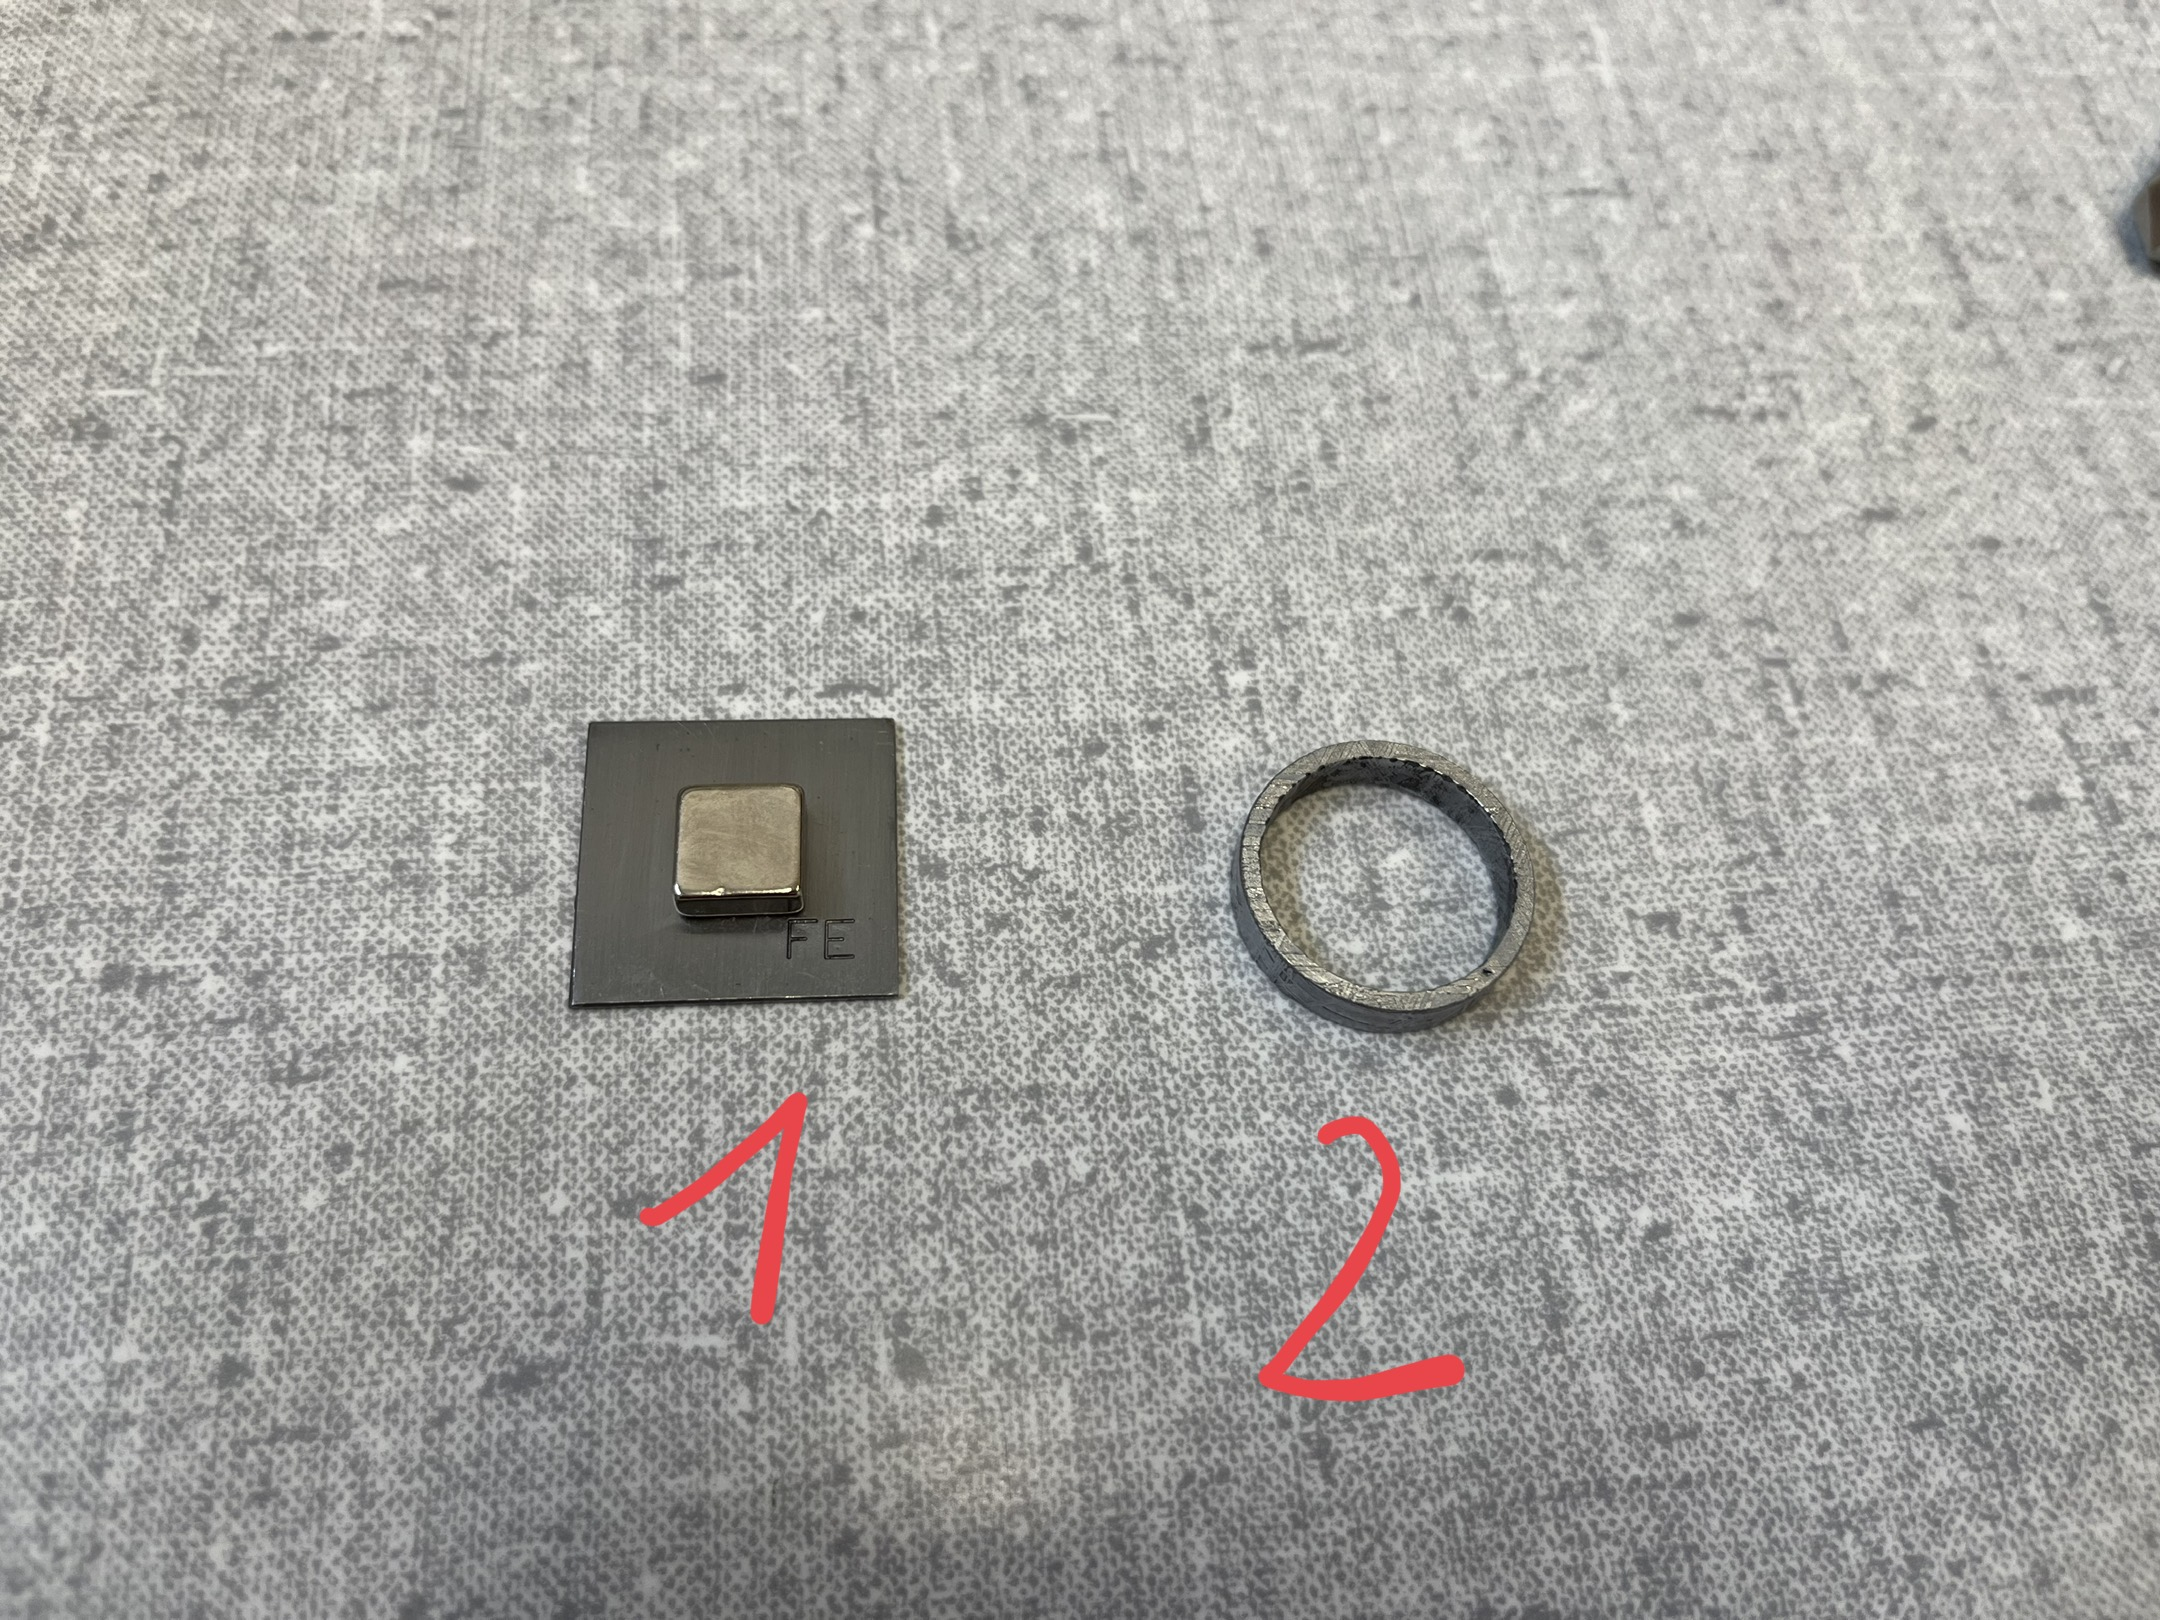
\includegraphics[width =0.8\textwidth]{./figures/eigene_proben.jpg}
	\end{center}
	\caption[Eigene Proben]
	{Eigene Proben\\
	1 \dots Neodynmagnet auf Eisenplättchen\\
	2 \dots Ring
	}\label{fig:unbekannte_pr}
\end{figure}

Um den Neodynmagneten besser auf dem Targethalter positionieren zu können, wurde dieser auf die Eisenplatte gegeben. Bei der
Auswertung ist nun zu beachten, dass diese Eisenplatte auch berücksichtigt werden muss.
Beim Ring ist zu Beachten dass bei der Positionierung darauf geachtet wurde, dass die Röntgenstrahlen den Ring auch 
wirklich treffen.

Die Messung der beiden Proben erfolgt nach dem gleichen Schema wie zuvor bei den Metallplättchen.
Die erzeugten Messungen sind in folgenden Abbildungen sichtbar.

%todo unbekannte proben

\subsection{Compton-Effekt}

\subsubsection{Energiekalibrierung des Detektors}

Nachdem das Röntgengerät wie bereits in \autoref{sec:versuchsanordnung} beschrieben vorbereitet wurde, indem
der Targetarm ausgebaut wird und Zr - Filter, sowie die Abschwächerblende positioniert wurden, wird zunächst der
Emissionsstrom auf \SI{0.05(2)}{mA} reduziert.
In der Cassy Lab Software werden die folgende Einstellungen vorgenommen: 
"Vielkanalmessung, 512 Kanäle, negative Pulse, Verstärkung = -4, Messdauer = 300 s“
Nun wird das Maximum der Zählrate bestimmt, indem eine Messung gestartet wird und der Sensor langsam um 
die 0°-Linie geschwenkt wird, bis das Maximum verzeichnet wird, was im konkreten Fall bei folgenden Winkel 
$\alpha_{max}$ der Fall war.

\begin{equation*}
	\alpha_{max} = \SI{-0.6(2)}{\degree}
\end{equation*}

Mit diesem Winkel wird eine gesammte Messperiode aufgezeichnet. Auch hier ist es wichtig darauf zu achten, dass die 
Tür ordnungsgemäß geschlossen ist.
Nun wird in der Computersoftware unter dem gleichnamigen Dialogfenster eine Energiekalibrierung durchgeführt,
indem die Energien für Au L$\alpha$ - \SI{9.71}{keV} und Mo K$\alpha$ - \SI{17.44}{keV} übergeben werden \cite{unterlagen_compton}.
Die so erzeugte Grafik ist in \autoref{fig:kalibrierung_compton} sichtbar.

%todo fig:kalibrierung_compton

\subsubsection{Aufnahme der Spektren bei verschiedenen Winkeln}

Nun wird, wie bereits in \autoref{sec:versuchsanordnung} beschrieben, die Abschwächerblende entfernt und
der Targethalter wieder Eingebaut. Auf diesen wirdvorsichtig die Plexiglasprobe gelegt.
Weiters wird wieder ein Emissionsstrom von \SI{1.00(2)}{mA} verwendet.
Nun wird der Targetarm über den entsprechenden Drehknopf um einen Winkel von \SI{20.0(2)}{\degree} geneigt und 
für alle Messungen in dieser Position belassen.
Für die verschiedenen Messungen wird nun der Neigungswinkel des Sensors variiert. Um den tatsächlichen Auslenkungswinkel
im Bezug zur Energiekalibrierung zu messen muss beachtet werden, dass der zuvor bestimmte Versatz von \SI{-0.6(2)}{\degree}
immer berücksichtigt wird. Eine tatsächliche Verdrehung des Sensors von \SI{30}{\degree} würde daher beispielsweise
einem Wert von \SI{29.4}{\degree} in der Anzeige entsprechen. Der besseren Übersicht halber, werden die Winkel in 
\autoref{tab:werte_compton} bezüglich der Kalibrierung angegeben. Nun wird in der Computersoftware über die peak-finder
Funktion die Energie des Peaks beim entsprechenden Abstrahlwinkel bestimmt und in \autoref{tab:werte_compton} notiert.


%todo tab:werte_compton

\section{Auswertung}\label{sec:auswertung}

Um zu sehen wie sich die Unsicherheit der Messungen bis in die Ergebnisse
fortpflanzt, ist erweiterte Gauss-Methode verwendet worden. Die Grundlagen
dieser Methode stammen von den Powerpointfolien von
GUM~\cite{wolfgang_kessel_isobipm-gum_2004}. Für die Auswertung ist die
Progammiersprache Python im speziellen die Pakete \verb#labtool-ex2#,
\verb#pandas#, \verb#sympy#, \verb#lmfit# zur Hilfe genommen worden.
\verb#lmfit# wurde für das Fitten verwendet, \verb#sympy# wurde für symbolische
Manipulation verwendet und die restlichen Pakete für leichteres Handhaben der
Daten. Dies wurde aber alles durch \verb#labtool-ex2# abstrahiert.

Um höchstmögliche Genauigkeit zu garantieren wird erst bei der Darstellung der
Wert in Tabellen gerundet.


\subsection{Röntgenfluoreszenzanalyse}

\subsubsection{bereitgestellte Metalle}


\subsubsection{unbekannte Probe}



\subsection{Compton-Effekt}

\subsubsection{Energiekalibrierung des Detektors}

\subsubsection{Aufnahme der Spektren bei verschiedenen Winkeln}

%todo bild mit sichtbarer verschiebung

\section{Diskussion}\label{sec:diskussion}

\subsection{Röntgenfluoreszenzanalyse}

\subsubsection{bereitgestellte Metalle}


\subsubsection{unbekannte Probe}

Um sicherzustellen, ob sich die Kalibration nicht verändert hat wurde zum Schluss nochmals die Fe Probe eingelegt
und der in \autoref{fig:fe_zumSchluss} sichtbare Energieverlauf erzeugt.

%todo fig:fe_zumSchluss

Hier wird klar ersichtlich, dass sich die Kalibrierung, wie erwartet, nicht geändert hat.

\subsection{Compton-Effekt}

\subsubsection{Energiekalibrierung des Detektors}

\subsubsection{Aufnahme der Spektren bei verschiedenen Winkeln}



\section{Zusammenfassung}\label{sec:zusammenfassung}

Hier werden nochmals alle Ergebnisse dieser Experimentenfolge aufgelistet.
Wobei die meisten zu erstellenden Diagramme Aufgrund der Länge der
\autoref{sec:auswertung} entnommen werden sollen.

\subsection{Röntgenfluoreszenzanalyse}

\subsubsection{bereitgestellte Metalle}


\subsubsection{unbekannte Probe}


\subsection{Compton-Effekt}

\subsubsection{Energiekalibrierung des Detektors}

\subsubsection{Aufnahme der Spektren bei verschiedenen Winkeln}


\newpage
\printbibliography
\listoffigures
\listoftables
\end{document}
